
\chapter{Stability: When Systems Blow Up}
\label{ch:stability}

\begin{quote}
\textit{``The notion of stability is really almost a trivial thing... A stable system is one which, when disturbed from its state of equilibrium, returns to that state; an unstable system is one which departs more and more from equilibrium when slightly displaced.''}

\hfill --- James Clerk Maxwell, ``On Governors'' (1868)
\end{quote}

\vspace{1em}

\noindent
Stability is perhaps the most fundamental concept in control systems engineering. An unstable system is not merely poorly performing---it is dangerous, potentially destructive, and fundamentally unusable. Before we can design controllers to achieve desired performance, we must first ensure that our systems will not ``blow up.'' This chapter develops the mathematical framework for analyzing stability and provides practical tools for determining whether a system is stable without solving the characteristic equation explicitly.

%=============================================================================
\section{Historical Motivation: The Quest for Stable Machines}
\label{sec:stability_history}
%=============================================================================

\subsection{James Watt and the Governor Problem}

The story of stability analysis begins with one of the most consequential inventions of the Industrial Revolution: James Watt's centrifugal governor for steam engines (circa 1788). While Watt did not invent the centrifugal mechanism---it had been used in windmills since the 1740s---he was the first to apply it to the critical problem of regulating steam engine speed.

The governor operated on an elegantly simple principle. Two weighted balls were attached to a vertical spindle connected to the engine's flywheel through a gear train. As the engine speed increased, centrifugal force caused the balls to swing outward and rise. This motion was linked through a lever mechanism to the steam throttle valve, reducing steam flow and thereby slowing the engine. Conversely, if the engine slowed, the balls dropped inward, opening the throttle and increasing power.

\begin{figure}[H]
\centering
\begin{tikzpicture}[scale=0.9]
  % Central spindle
  \draw[thick] (0,0) -- (0,4);
  \draw[thick,fill=gray!30] (-0.15,0) rectangle (0.15,0.3);

  % Arms and balls - normal position
  \draw[thick] (0,3) -- (-1.2,2) node[circle,fill=black,minimum size=8pt,inner sep=0pt] (ball1) {};
  \draw[thick] (0,3) -- (1.2,2) node[circle,fill=black,minimum size=8pt,inner sep=0pt] (ball2) {};

  % Arms extended position (dashed)
  \draw[thick,dashed,gray] (0,3) -- (-1.8,2.8);
  \draw[thick,dashed,gray] (0,3) -- (1.8,2.8);
  \draw[dashed,gray] (-1.8,2.8) node[circle,draw,minimum size=8pt,inner sep=0pt] {};
  \draw[dashed,gray] (1.8,2.8) node[circle,draw,minimum size=8pt,inner sep=0pt] {};

  % Collar and linkage
  \draw[thick,fill=gray!50] (-0.3,1.5) rectangle (0.3,1.8);
  \draw[thick] (-1.2,2) -- (-0.3,1.65);
  \draw[thick] (1.2,2) -- (0.3,1.65);

  % Throttle linkage
  \draw[thick] (0.3,1.65) -- (1.5,1.65) -- (1.5,0.5);
  \draw[thick,fill=white] (1.3,0.3) rectangle (1.7,0.7);
  \node[right] at (1.8,0.5) {\small Throttle};

  % Rotation arrow
  \draw[-{Stealth},thick] (0.5,3.5) arc (0:270:0.5);
  \node at (0,4.3) {\small $\omega$};

  % Labels
  \node[left] at (-1.5,2) {\small Flyball};
  \node[above] at (0,3.2) {\small Spindle};

  % Annotation for hunting
  \draw[<->,red,thick] (-2.2,2) -- (-2.2,2.8);
  \node[red,left] at (-2.2,2.4) {\small Hunting};
\end{tikzpicture}
\caption{Watt's centrifugal governor. Dashed lines show extended position at higher speed. ``Hunting'' oscillations occur when the system becomes marginally stable.}
\label{fig:watt_governor}
\end{figure}

For decades, Watt governors worked adequately, but as steam engines grew larger and more powerful in the mid-19th century, a troubling phenomenon emerged: \textbf{hunting}. Instead of settling to a steady speed, some governors would oscillate continuously. The engine would speed up, causing the governor to close the throttle, which slowed the engine, causing the governor to open the throttle, which sped up the engine---an endless cycle that made precise control impossible and wore out machinery prematurely.

The hunting problem was not merely an annoyance; it represented a fundamental limitation on the size and power of controllable steam engines. Engineers of the era struggled to understand why some governors worked perfectly while others, seemingly identical in design, oscillated uncontrollably.

\subsection{Maxwell's ``On Governors'' (1868)}

\begin{historicalbox}[Maxwell and the Birth of Control Theory]
The breakthrough came from an unlikely source: James Clerk Maxwell, already famous for unifying electricity and magnetism, turned his attention to the governor problem in 1868. His paper ``On Governors,'' published in the Proceedings of the Royal Society of London, is now recognized as the founding document of control theory.

Maxwell approached the problem with the tools of mathematical physics. He wrote the equations of motion for the governor-engine system as a set of linear differential equations and asked: under what conditions do small disturbances die out over time? This was the first rigorous formulation of the stability problem.

Maxwell showed that the behavior of the system depended on the roots of a characteristic equation---a polynomial whose coefficients were determined by the physical parameters of the governor and engine. If all roots had negative real parts, disturbances would decay exponentially and the system was stable. If any root had a positive real part, disturbances would grow exponentially: instability.

For second and third-order systems, Maxwell derived explicit conditions on the coefficients that guaranteed stability. But he noted that for higher-order systems, determining whether all roots lay in the left half-plane was a difficult algebraic problem. He posed this as a challenge to mathematicians:

\begin{quote}
\textit{``The great difficulty of this theory lies in the determination of the conditions of stability of the motion... I am not aware of any method of determining the nature of the roots of an equation of a higher degree than the third.''}
\end{quote}
\end{historicalbox}

\subsection{Routh's Criterion (1877)}

Maxwell's challenge was answered by Edward John Routh, a Cambridge mathematician who had been Maxwell's fellow student (and actually beat Maxwell for the prestigious Smith's Prize in 1854). In 1877, Routh published ``A Treatise on the Stability of a Given State of Motion,'' which provided a complete algorithmic solution to the stability problem.

Routh developed a systematic procedure---now called the \textbf{Routh array} or \textbf{Routh table}---that could determine the number of roots with positive real parts for a polynomial of any degree, without actually solving the polynomial. The method required only arithmetic operations on the coefficients, making it practical for hand calculation even for high-order systems.

For this work, Routh received the Adams Prize from Cambridge in 1877. His criterion became the standard tool for stability analysis in British engineering for the next century.

\subsection{Hurwitz's Independent Discovery (1895)}

In 1895, the German mathematician Adolf Hurwitz independently developed equivalent stability conditions while studying a completely different problem in pure mathematics (the theory of continued fractions). Hurwitz expressed his conditions in terms of determinants of matrices formed from the polynomial coefficients.

When the connection between Routh's and Hurwitz's work was recognized, the combined result became known as the \textbf{Routh-Hurwitz stability criterion}. It remains one of the most important tools in control engineering, despite the availability of powerful computers that can find polynomial roots directly.

\subsection{Dramatic Failures: Lessons in Instability}

\subsubsection{The Tacoma Narrows Bridge (1940)}

On November 7, 1940, the Tacoma Narrows Bridge in Washington State collapsed in a spectacular fashion, captured on film that has since been viewed by millions of engineering students. The bridge, nicknamed ``Galloping Gertie'' for its tendency to oscillate in the wind, exhibited increasingly violent torsional oscillations in a 40 mph wind before tearing itself apart.

\begin{figure}[H]
\centering
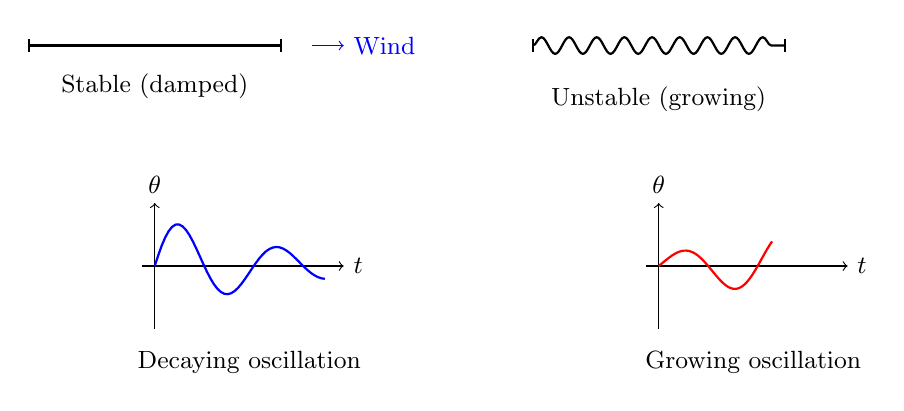
\begin{tikzpicture}[scale=0.8]
  % Bridge deck representations
  % Stable
  \begin{scope}[shift={(-4,2)}]
    \draw[thick] (-2,0) -- (2,0);
    \draw[thick] (-2,-0.1) -- (-2,0.1);
    \draw[thick] (2,-0.1) -- (2,0.1);
    \node[below] at (0,-0.3) {\small Stable (damped)};
    \draw[->,blue] (2.5,0) -- (3,0);
    \node[blue,right] at (3,0) {\small Wind};
  \end{scope}

  % Oscillating
  \begin{scope}[shift={(4,2)}]
    \draw[thick,decorate,decoration={snake,amplitude=3pt,segment length=10pt}] (-2,0) -- (2,0);
    \draw[thick] (-2,-0.1) -- (-2,0.1);
    \draw[thick] (2,-0.1) -- (2,0.1);
    \node[below] at (0,-0.5) {\small Unstable (growing)};
  \end{scope}

  % Time response plots
  \begin{scope}[shift={(-4,-1.5)}]
    \draw[->] (-0.2,0) -- (3,0) node[right] {\small $t$};
    \draw[->] (0,-1) -- (0,1) node[above] {\small $\theta$};
    \draw[blue,thick,domain=0:2.7,samples=50] plot (\x,{0.8*exp(-0.5*\x)*sin(4*\x r)});
    \node[below] at (1.5,-1.2) {\small Decaying oscillation};
  \end{scope}

  \begin{scope}[shift={(4,-1.5)}]
    \draw[->] (-0.2,0) -- (3,0) node[right] {\small $t$};
    \draw[->] (0,-1) -- (0,1) node[above] {\small $\theta$};
    \draw[red,thick,domain=0:1.8,samples=50] plot (\x,{0.2*exp(0.5*\x)*sin(4*\x r)});
    \node[below] at (1.5,-1.2) {\small Growing oscillation};
  \end{scope}
\end{tikzpicture}
\caption{Bridge deck oscillation modes. Left: stable, damped response. Right: unstable, growing oscillation as occurred at Tacoma Narrows.}
\label{fig:tacoma}
\end{figure}

The collapse is often incorrectly attributed to resonance---the wind frequency matching a natural frequency of the bridge. Modern analysis reveals that the actual mechanism was \textbf{aeroelastic flutter}, a self-excited instability. The bridge's motion modified the aerodynamic forces in a way that extracted energy from the wind, feeding the oscillations. This is a classic feedback instability: the output (bridge motion) affected the input (aerodynamic forces) in a destabilizing manner.

\subsubsection{Early Aircraft Instabilities}

The Wright brothers' 1903 Flyer was actually designed to be inherently unstable in pitch. The brothers reasoned that this would make the aircraft more maneuverable---and they were right, but it also meant the pilot had to constantly work to maintain level flight. Later aviators, less skilled than the Wrights, crashed repeatedly trying to fly unstable aircraft.

Several forms of instability plagued early aviation. \textbf{Spiral instability} occurs when a slight bank angle leads to a sideslip, which increases the bank, leading to an ever-tightening spiral dive; many early aviators, flying in clouds without visual references, died in spiral dives. \textbf{Dutch roll} is a coupled yaw-roll oscillation where the nose swings left-right while the wings rock side-to-side, and while mildly unstable Dutch roll merely makes passengers airsick, severely unstable Dutch roll can be completely uncontrollable. \textbf{Pilot-induced oscillation (PIO)} occurs when the pilot, reacting to aircraft motion with a slight time delay, actually destabilizes the system through the feedback loop: pilot $\to$ controls $\to$ aircraft $\to$ pilot. This phenomenon has caused crashes of advanced aircraft including early fly-by-wire prototypes.

These historical examples underscore a crucial lesson: stability is not an academic abstraction but a matter of life and death in real engineering systems.

%=============================================================================
\section{Modern Applications of Stability Theory}
\label{sec:modern_applications}
%=============================================================================

Stability analysis remains central to modern engineering across diverse domains:

\subsection{Power Grid Stability}

The electric power grid is one of the largest and most complex dynamic systems ever built. Thousands of generators must rotate in precise synchronism at 60 Hz (in North America) or 50 Hz (in Europe). Loss of synchronism leads to \textbf{blackouts} affecting millions of people.

The 2003 Northeast Blackout, which affected 55 million people, was triggered by a relatively minor fault (high-voltage lines sagging into trees in Ohio). The fault caused a cascading failure because the system's stability margins were insufficient to absorb the disturbance. Modern grid operators use sophisticated stability analysis to maintain adequate margins and plan for contingencies.

\subsection{Flight Control: Intentionally Unstable Aircraft}

Modern fighter aircraft like the F-16, F-22, and Eurofighter are designed to be \textbf{inherently unstable} in certain flight regimes. An unstable aircraft, by definition, will depart from level flight if left alone---but this instability provides extraordinary maneuverability. The aircraft can change direction faster than a stable design because it ``wants'' to move.

This approach is only possible with active control. Flight computers, sampling sensors hundreds of times per second, continuously adjust control surfaces to maintain stability. If the flight control computer fails, the pilot has only seconds before the aircraft becomes uncontrollable. This ``relaxed static stability'' design trades passive safety for performance, with the risk managed by redundant computers and extensive testing.

The B-2 stealth bomber carries this concept further. Its flying-wing design, optimized for low radar cross-section, is unstable in multiple axes. Without the flight control system, the B-2 cannot fly.

\subsection{Audio Feedback}

The familiar ``squeal'' when a microphone is placed too close to its speaker is an example of instability in an acoustic feedback loop:
\[
\text{Microphone} \to \text{Amplifier} \to \text{Speaker} \to \text{(acoustic path)} \to \text{Microphone}
\]
If the loop gain (amplifier gain times acoustic coupling) exceeds unity at any frequency where the phase shift equals a multiple of $360°$, the Barkhausen criterion for oscillation is satisfied, and the system becomes unstable at that frequency. Sound engineers use equalization (reducing gain at problematic frequencies) and careful microphone placement to maintain stability.

\subsection{Economic and Financial Stability}

Economic systems exhibit feedback dynamics: interest rate changes affect borrowing, which affects spending, which affects inflation, which affects interest rates. Central banks attempt to stabilize economies by adjusting monetary policy, but time delays and nonlinearities make this challenging.

Financial markets can exhibit instability through feedback mechanisms like portfolio insurance (selling during declines) and margin calls (forced selling when prices fall), which amplify price movements. The 1987 stock market crash, when the Dow Jones Industrial Average fell 22\% in a single day, has been attributed partly to such destabilizing feedback.

%=============================================================================
\section{Mathematical Foundation of Stability}
\label{sec:math_foundation}
%=============================================================================

We now develop the rigorous mathematical theory of stability for linear time-invariant (LTI) systems.

\subsection{BIBO Stability: Definition}

\begin{definition}[BIBO Stability]
\label{def:bibo}
A system is \textbf{Bounded-Input Bounded-Output (BIBO) stable} if and only if every bounded input produces a bounded output. Formally, if there exists $M < \infty$ such that $|u(t)| \leq M$ for all $t \geq 0$, then there exists $N < \infty$ such that $|y(t)| \leq N$ for all $t \geq 0$.
\end{definition}

This definition captures the intuitive notion of a ``well-behaved'' system. A BIBO-stable system cannot produce unbounded outputs from bounded inputs; it cannot ``blow up'' in response to reasonable excitation.

\subsection{Impulse Response and Stability}

For an LTI system with impulse response $h(t)$, the output $y(t)$ in response to input $u(t)$ is given by the convolution integral:
\begin{equation}
y(t) = \int_0^t h(\tau) u(t-\tau) \, d\tau = \int_0^t h(t-\tau) u(\tau) \, d\tau
\label{eq:convolution}
\end{equation}

\begin{theorem}[Impulse Response Criterion for BIBO Stability]
\label{thm:impulse_stability}
An LTI system is BIBO stable if and only if its impulse response is absolutely integrable:
\begin{equation}
\int_0^\infty |h(t)| \, dt < \infty
\label{eq:absolute_integrable}
\end{equation}
\end{theorem}

\begin{proof}
\textbf{(Sufficiency)} Suppose $\int_0^\infty |h(t)| \, dt = H < \infty$ and $|u(t)| \leq M$ for all $t$. Then:
\begin{align}
|y(t)| &= \left| \int_0^t h(\tau) u(t-\tau) \, d\tau \right| \\
&\leq \int_0^t |h(\tau)| |u(t-\tau)| \, d\tau \\
&\leq M \int_0^t |h(\tau)| \, d\tau \\
&\leq M \int_0^\infty |h(\tau)| \, d\tau = MH
\end{align}
Thus $|y(t)| \leq MH < \infty$, proving the output is bounded.

\textbf{(Necessity)} Suppose $\int_0^\infty |h(t)| \, dt = \infty$. We construct a bounded input that produces an unbounded output. Define:
\begin{equation}
u(t) = \begin{cases}
+1 & \text{if } h(T-t) \geq 0 \\
-1 & \text{if } h(T-t) < 0
\end{cases}
\end{equation}
for some fixed $T > 0$. This input is clearly bounded: $|u(t)| \leq 1$. The output at time $T$ is:
\begin{equation}
y(T) = \int_0^T h(\tau) u(T-\tau) \, d\tau = \int_0^T |h(\tau)| \, d\tau
\end{equation}
As $T \to \infty$, we have $y(T) \to \int_0^\infty |h(\tau)| \, d\tau = \infty$. Thus the output is unbounded.
\end{proof}

\subsection{Pole Location Criterion}

For rational transfer functions, there is an elegant connection between BIBO stability and the location of poles in the complex $s$-plane.

\begin{theorem}[Pole Location Criterion]
\label{thm:pole_location}
A system with rational transfer function $G(s)$ is BIBO stable if and only if all poles of $G(s)$ lie in the open left half-plane (LHP), i.e., all poles have strictly negative real parts.
\end{theorem}

\begin{figure}[H]
\centering
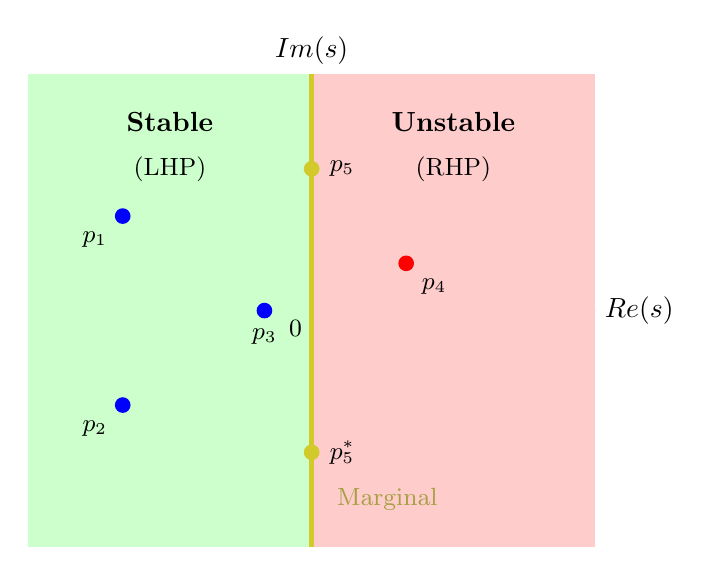
\begin{tikzpicture}[scale=1.2]
  % Axes
  \draw[->] (-3,0) -- (3,0) node[right] {$\text{Re}(s)$};
  \draw[->] (0,-2.5) -- (0,2.5) node[above] {$\text{Im}(s)$};

  % Left half plane (stable region)
  \fill[green!20] (-3,-2.5) rectangle (0,2.5);

  % Right half plane (unstable region)
  \fill[red!20] (0,-2.5) rectangle (3,2.5);

  % Imaginary axis (marginal)
  \draw[yellow!80!black,line width=2pt] (0,-2.5) -- (0,2.5);

  % Labels
  \node at (-1.5,2) {\textbf{Stable}};
  \node at (-1.5,1.5) {\small (LHP)};
  \node at (1.5,2) {\textbf{Unstable}};
  \node at (1.5,1.5) {\small (RHP)};
  \node[yellow!60!black] at (0.8,-2) {\small Marginal};

  % Example poles - stable
  \node[circle,fill=blue,inner sep=2pt,label=below left:{\small $p_1$}] at (-2,1) {};
  \node[circle,fill=blue,inner sep=2pt,label=below left:{\small $p_2$}] at (-2,-1) {};
  \node[circle,fill=blue,inner sep=2pt,label=below:{\small $p_3$}] at (-0.5,0) {};

  % Example poles - unstable
  \node[circle,fill=red,inner sep=2pt,label=below right:{\small $p_4$}] at (1,0.5) {};

  % Example pole - marginal
  \node[circle,fill=yellow!80!black,inner sep=2pt,label=right:{\small $p_5$}] at (0,1.5) {};
  \node[circle,fill=yellow!80!black,inner sep=2pt,label=right:{\small $p_5^*$}] at (0,-1.5) {};

  % Origin
  \node[below left] at (0,0) {\small $0$};
\end{tikzpicture}
\caption{The $s$-plane divided into stable, unstable, and marginally stable regions. Poles $p_1$, $p_2$, $p_3$ (LHP) correspond to stable modes. Pole $p_4$ (RHP) causes instability. Poles $p_5$, $p_5^*$ (imaginary axis) produce sustained oscillations---marginal stability.}
\label{fig:s_plane_regions}
\end{figure}

\begin{proof}
Consider a transfer function with partial fraction expansion:
\begin{equation}
G(s) = \sum_{i=1}^n \frac{r_i}{s - p_i}
\end{equation}
where $p_i$ are the poles (assumed distinct for simplicity) and $r_i$ are the residues. The impulse response is:
\begin{equation}
h(t) = \mathcal{L}^{-1}\{G(s)\} = \sum_{i=1}^n r_i e^{p_i t}, \quad t \geq 0
\end{equation}

For a pole $p_i = \sigma_i + j\omega_i$, the behavior depends on the sign of the real part. When $\sigma_i < 0$ (LHP pole), $|e^{p_i t}| = e^{\sigma_i t} \to 0$ as $t \to \infty$, so this term decays exponentially. When $\sigma_i > 0$ (RHP pole), $|e^{p_i t}| = e^{\sigma_i t} \to \infty$ as $t \to \infty$, causing this term to grow exponentially. When $\sigma_i = 0$ (imaginary axis), $|e^{p_i t}| = 1$ for all $t$, so this term neither grows nor decays.

For BIBO stability, we need $\int_0^\infty |h(t)| \, dt < \infty$. The integral of $e^{\sigma t}$ is:
\begin{equation}
\int_0^\infty e^{\sigma t} \, dt = \begin{cases}
-1/\sigma < \infty & \text{if } \sigma < 0 \\
\infty & \text{if } \sigma \geq 0
\end{cases}
\end{equation}
Therefore, absolute integrability (and thus BIBO stability) requires all poles to have $\sigma_i < 0$, i.e., all poles in the open LHP.
\end{proof}

\begin{figure}[H]
\centering
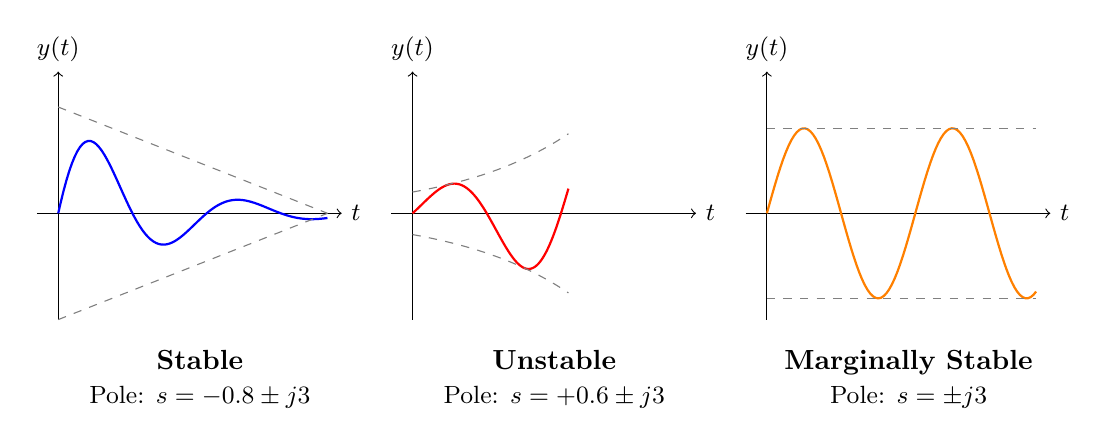
\begin{tikzpicture}[scale=0.9]
  % Stable response
  \begin{scope}[shift={(-5,0)}]
    \draw[->] (-0.3,0) -- (4,0) node[right] {\small $t$};
    \draw[->] (0,-1.5) -- (0,2) node[above] {\small $y(t)$};
    \draw[blue,thick,domain=0:3.8,samples=100] plot (\x,{1.5*exp(-0.8*\x)*sin(3*\x r)});
    \draw[dashed,gray] (0,1.5) -- (3.8,0);
    \draw[dashed,gray] (0,-1.5) -- (3.8,0);
    \node[below] at (2,-1.8) {\textbf{Stable}};
    \node[below] at (2,-2.3) {\small Pole: $s = -0.8 \pm j3$};
  \end{scope}

  % Unstable response
  \begin{scope}[shift={(0,0)}]
    \draw[->] (-0.3,0) -- (4,0) node[right] {\small $t$};
    \draw[->] (0,-1.5) -- (0,2) node[above] {\small $y(t)$};
    \draw[red,thick,domain=0:2.2,samples=100] plot (\x,{0.3*exp(0.6*\x)*sin(3*\x r)});
    \draw[dashed,gray,domain=0:2.2] plot (\x,{0.3*exp(0.6*\x)});
    \draw[dashed,gray,domain=0:2.2] plot (\x,{-0.3*exp(0.6*\x)});
    \node[below] at (2,-1.8) {\textbf{Unstable}};
    \node[below] at (2,-2.3) {\small Pole: $s = +0.6 \pm j3$};
  \end{scope}

  % Marginally stable
  \begin{scope}[shift={(5,0)}]
    \draw[->] (-0.3,0) -- (4,0) node[right] {\small $t$};
    \draw[->] (0,-1.5) -- (0,2) node[above] {\small $y(t)$};
    \draw[orange,thick,domain=0:3.8,samples=100] plot (\x,{1.2*sin(3*\x r)});
    \draw[dashed,gray] (0,1.2) -- (3.8,1.2);
    \draw[dashed,gray] (0,-1.2) -- (3.8,-1.2);
    \node[below] at (2,-1.8) {\textbf{Marginally Stable}};
    \node[below] at (2,-2.3) {\small Pole: $s = \pm j3$};
  \end{scope}
\end{tikzpicture}
\caption{Time responses corresponding to different pole locations. Stable poles (LHP) produce decaying responses. Unstable poles (RHP) produce growing responses. Imaginary axis poles produce sustained oscillations.}
\label{fig:time_responses}
\end{figure}

\subsection{Marginal Stability}

\begin{definition}[Marginal Stability]
A system is \textbf{marginally stable} if it is not BIBO stable, but its impulse response remains bounded (though not necessarily decaying) for all time.
\end{definition}

Marginal stability occurs when there are poles on the imaginary axis (simple poles only---repeated imaginary poles cause unbounded growth). A marginally stable system will oscillate indefinitely in response to an impulse but will not grow without bound.

\begin{warningbox}[Engineering Caution]
Marginally stable systems are unacceptable in most engineering applications. While mathematically the response is bounded, several practical concerns arise. First, any modeling error could place poles slightly in the RHP, causing instability. Second, nonlinearities not captured by the linear model may cause limit cycles or chaos. Third, sustained oscillations waste energy and cause mechanical wear. For these reasons, a well-designed system should have all poles strictly in the LHP with adequate stability margins.
\end{warningbox}

\subsection{Closed-Loop Stability}

For a feedback system with forward path $G(s)$ and feedback path $H(s)$, the closed-loop transfer function is:
\begin{equation}
T(s) = \frac{G(s)}{1 + G(s)H(s)}
\label{eq:closed_loop}
\end{equation}

\begin{figure}[H]
\centering
\begin{tikzpicture}[auto, node distance=2cm,>=Stealth]
  % Blocks
  \node[draw, circle, inner sep=1.5pt] (sum) at (0,0) {$\Sigma$};
  \node[draw, rectangle, minimum width=1.2cm, minimum height=0.8cm] (G) at (2.5,0) {$G(s)$};
  \node[draw, rectangle, minimum width=1.2cm, minimum height=0.8cm] (H) at (2.5,-1.5) {$H(s)$};

  % Connections
  \draw[->] (-2,0) -- node[pos=0.3,above] {$R(s)$} (sum);
  \draw[->] (sum) -- node[above] {$E(s)$} (G);
  \draw[->] (G) -- (4.5,0) node[right] {$Y(s)$};
  \draw[->] (3.8,0) |- (H);
  \draw[->] (H) -| node[pos=0.9,left] {$-$} (sum);

  % Plus sign
  \node[above left] at (sum.north west) {\small $+$};
\end{tikzpicture}
\caption{Standard feedback configuration. The closed-loop poles are roots of $1 + G(s)H(s) = 0$.}
\label{fig:feedback_block}
\end{figure}

The closed-loop poles are the roots of the \textbf{characteristic equation}:
\begin{equation}
1 + G(s)H(s) = 0
\label{eq:characteristic}
\end{equation}

\begin{conceptbox}[Key Insight: Open-Loop vs. Closed-Loop Stability]
The open-loop transfer function $G(s)H(s)$ and closed-loop transfer function $T(s)$ generally have \emph{different} poles. A system can be open-loop stable but closed-loop unstable when too much gain is applied, or it can be open-loop unstable but closed-loop stable through feedback stabilization. Stability analysis must therefore focus on the \emph{closed-loop} poles, which are roots of the characteristic equation $1 + G(s)H(s) = 0$.
\end{conceptbox}

%=============================================================================
\section{The Routh-Hurwitz Stability Criterion}
\label{sec:routh_hurwitz}
%=============================================================================

The Routh-Hurwitz criterion provides a method to determine how many roots of a polynomial lie in the right half-plane without actually solving for the roots. This is invaluable for stability analysis, especially when the polynomial coefficients depend on design parameters.

\subsection{The Routh Array}

Consider a polynomial of degree $n$:
\begin{equation}
P(s) = a_n s^n + a_{n-1} s^{n-1} + a_{n-2} s^{n-2} + \cdots + a_1 s + a_0
\label{eq:characteristic_poly}
\end{equation}

\begin{theorem}[Necessary Condition for Stability]
\label{thm:necessary}
A necessary (but not sufficient) condition for all roots of $P(s)$ to have negative real parts is that all coefficients $a_i$ have the same sign and are nonzero.
\end{theorem}

If any coefficient is zero or has a different sign, there is at least one root with non-negative real part. However, all coefficients being positive does not guarantee stability for polynomials of degree 3 or higher.

\begin{definition}[Routh Array]
The Routh array is a triangular table constructed from the polynomial coefficients as follows:

\begin{center}
\begin{tabular}{c|ccccc}
$s^n$ & $a_n$ & $a_{n-2}$ & $a_{n-4}$ & $a_{n-6}$ & $\cdots$ \\
$s^{n-1}$ & $a_{n-1}$ & $a_{n-3}$ & $a_{n-5}$ & $a_{n-7}$ & $\cdots$ \\
$s^{n-2}$ & $b_1$ & $b_2$ & $b_3$ & $b_4$ & $\cdots$ \\
$s^{n-3}$ & $c_1$ & $c_2$ & $c_3$ & $c_4$ & $\cdots$ \\
$\vdots$ & $\vdots$ & $\vdots$ & $\vdots$ & $\vdots$ & \\
$s^1$ & $*$ & & & & \\
$s^0$ & $*$ & & & & \\
\end{tabular}
\end{center}

where the elements are computed using:
\begin{align}
b_1 &= \frac{a_{n-1} \cdot a_{n-2} - a_n \cdot a_{n-3}}{a_{n-1}} \\
b_2 &= \frac{a_{n-1} \cdot a_{n-4} - a_n \cdot a_{n-5}}{a_{n-1}} \\
c_1 &= \frac{b_1 \cdot a_{n-3} - a_{n-1} \cdot b_2}{b_1}
\end{align}
and so on, with each element computed from the two rows immediately above it.
\end{definition}

The general formula for an element in row $i$, column $j$ is:
\begin{equation}
\text{element}_{i,j} = \frac{(\text{first element of row } i-1) \times (\text{element } j+1 \text{ of row } i-2) - (\text{first element of row } i-2) \times (\text{element } j+1 \text{ of row } i-1)}{\text{first element of row } i-1}
\end{equation}

\begin{theorem}[Routh-Hurwitz Criterion]
\label{thm:routh}
The number of roots of $P(s)$ in the right half-plane equals the number of sign changes in the first column of the Routh array.
\end{theorem}

\begin{corollary}
A polynomial has all roots in the left half-plane (and hence the corresponding system is stable) if and only if all elements in the first column of the Routh array have the same sign.
\end{corollary}

\subsection{Special Cases}

Two special situations require modified procedures:

\subsubsection{Case 1: Zero in the First Column (Other Elements Non-Zero)}

If a zero appears in the first column but other elements in that row are nonzero, replace the zero with a small positive number $\epsilon$ and continue the array construction. After completing the array, examine the signs as $\epsilon \to 0^+$.

\subsubsection{Case 2: Entire Row of Zeros}

A row of zeros indicates the presence of pairs of roots that are symmetric about the origin: either a pair of real roots at $\pm\sigma$, a pair of imaginary roots at $\pm j\omega$, or a quadruplet at $\pm\sigma \pm j\omega$.

The procedure for handling a row of zeros involves forming the \textbf{auxiliary polynomial} $A(s)$ from the row immediately above the zero row. The roots of $A(s)$ are among the symmetric root pairs. Next, replace the zero row with coefficients obtained from the derivative $\frac{dA}{ds}$, and then continue the Routh array construction normally.

%=============================================================================
\section{Practical Experiment: Demonstrating Stability and Instability}
\label{sec:experiment}
%=============================================================================

Understanding stability through hands-on experimentation provides intuition that mathematics alone cannot convey. This section presents a practical laboratory exercise using an op-amp circuit that can be configured for stable operation, marginal stability (oscillation), or instability.

\begin{experimentbox}[Laboratory Exercise: Op-Amp Feedback Stability]
\textbf{Objective:} Observe the effect of feedback on system stability by building an adjustable-gain feedback circuit and measuring its response as gain increases through the stability boundary.

\textbf{Learning Outcomes:} Upon completing this exercise, students will be able to observe stable, marginally stable, and unstable behavior in a real system, correlate mathematical stability criteria with physical behavior, and understand gain margins and their practical significance.
\end{experimentbox}

\subsection{Circuit Description}

We construct a second-order system using two op-amp integrators in a feedback loop with adjustable gain.

\begin{figure}[H]
\centering
\begin{circuitikz}[american, scale=0.85, transform shape]
  % First integrator
  \draw (0,0) node[op amp, yscale=-1] (opamp1) {};
  \draw (opamp1.-) -- ++(-0.5,0) to[R, l=$R_1$] ++(-2,0) node[left] {$v_{in}$};
  \draw (opamp1.-) -- ++(0,1.5) to[C, l=$C_1$] ++(2,0) -| (opamp1.out);
  \draw (opamp1.+) -- ++(0,-0.5) node[ground] {};
  \draw (opamp1.out) -- ++(0.5,0) node[right] {$v_1$};

  % Second integrator
  \draw (5,0) node[op amp, yscale=-1] (opamp2) {};
  \draw (opamp1.out) -- ++(0.5,0) to[R, l=$R_2$] (opamp2.-);
  \draw (opamp2.-) -- ++(0,1.5) to[C, l=$C_2$] ++(2,0) -| (opamp2.out);
  \draw (opamp2.+) -- ++(0,-0.5) node[ground] {};

  % Feedback path with potentiometer
  \draw (opamp2.out) -- ++(1,0) node[right] {$v_{out}$};
  \draw (opamp2.out) ++(0.5,0) -- ++(0,-2.5) to[pR, l=$K$ (pot)] ++(-7,0) -- ++(0,1) to[R, l=$R_f$] ++(0,1.5);
  \draw (-2.5,0) to[short] (opamp1.-);

  % Labels
  \node at (0,-2.5) {\small Integrator 1};
  \node at (5,-2.5) {\small Integrator 2};
\end{circuitikz}
\caption{Two-integrator oscillator/unstable system. Adjusting potentiometer $K$ changes the feedback gain, transitioning the system through stable, marginally stable, and unstable regions.}
\label{fig:circuit}
\end{figure}

The transfer function of this system (from $v_{in}$ to $v_{out}$) is:
\begin{equation}
G(s) = \frac{1}{(R_1C_1)(R_2C_2)s^2 + K}
\end{equation}

The characteristic equation is:
\begin{equation}
\tau_1\tau_2 s^2 + K = 0 \quad \Rightarrow \quad s^2 = -\frac{K}{\tau_1\tau_2}
\end{equation}
where $\tau_1 = R_1C_1$ and $\tau_2 = R_2C_2$.

The system behavior depends critically on the feedback gain $K$. For $K > 0$, the poles lie at $s = \pm j\sqrt{K/(\tau_1\tau_2)}$ on the imaginary axis, producing marginal stability with sustained oscillation. For $K < 0$ (positive feedback), the poles move to $s = \pm\sqrt{|K|/(\tau_1\tau_2)}$ on the real axis, placing one pole in the RHP and causing instability. Adding damping through a resistor in parallel with the capacitors moves the poles into the LHP, achieving stability.

\subsection{Alternative: Arduino-Based Motor Control Experiment}

For a more dynamic demonstration, we can use an Arduino microcontroller to implement digital feedback control of a DC motor.

\begin{figure}[H]
\centering
\begin{tikzpicture}[node distance=1.8cm, auto, >=Stealth, scale=0.9, transform shape]
  % Blocks
  \node[draw, rectangle, minimum width=2cm, minimum height=1cm] (arduino) {Arduino};
  \node[draw, rectangle, minimum width=1.5cm, minimum height=1cm, right=of arduino] (driver) {Motor Driver};
  \node[draw, rectangle, minimum width=1.5cm, minimum height=1cm, right=of driver] (motor) {DC Motor};
  \node[draw, rectangle, minimum width=1.5cm, minimum height=1cm, below=1.2cm of motor] (encoder) {Encoder};

  % Connections
  \draw[->] (arduino) -- node[above] {\small PWM} (driver);
  \draw[->] (driver) -- node[above] {\small Power} (motor);
  \draw[->] (motor) -- (encoder);
  \draw[->] (encoder) -| node[pos=0.3,below] {\small Position feedback} (arduino);

  % Setpoint
  \draw[->] (-2,0) -- node[above] {\small Setpoint} (arduino);
\end{tikzpicture}
\caption{Arduino-based motor position control system for stability demonstration.}
\label{fig:arduino_system}
\end{figure}

\begin{algorithm}[H]
\caption{Motor Position Control with Adjustable Gain}
\label{alg:motor_control}
\begin{algorithmic}[1]
\State \textbf{Initialize:}
\State \hspace{1em} Configure PWM output pin and direction pin
\State \hspace{1em} Configure encoder input pins with interrupts
\State \hspace{1em} Set $\textit{encoderCount} \gets 0$
\State \hspace{1em} Set $\textit{setpoint} \gets 0$
\State \hspace{1em} Set $K_p \gets 1.0$ \Comment{Proportional gain}
\State
\State \textbf{Main Control Loop:}
\While{system is running}
    \If{command received from user interface}
        \If{command is ``set gain''}
            \State $K_p \gets \text{new gain value}$
        \ElsIf{command is ``set position''}
            \State $\textit{setpoint} \gets \text{new position value}$
        \EndIf
    \EndIf
    \State
    \State \Comment{Proportional controller calculation}
    \State $\textit{error} \gets \textit{setpoint} - \textit{encoderCount}$
    \State $\textit{output} \gets K_p \times \textit{error}$
    \State
    \State \Comment{Apply control signal to motor}
    \State $\textit{pwm} \gets \min(\max(|\textit{output}|, 0), 255)$
    \State Set motor direction based on $\text{sign}(\textit{output})$
    \State Apply PWM signal to motor driver
    \State
    \State \Comment{Log data for analysis}
    \State Output: timestamp, setpoint, encoderCount
    \State Wait for next control cycle (10 ms period)
\EndWhile
\State
\State \textbf{Encoder Interrupt Handler:}
\If{encoder channel B is high}
    \State $\textit{encoderCount} \gets \textit{encoderCount} + 1$
\Else
    \State $\textit{encoderCount} \gets \textit{encoderCount} - 1$
\EndIf
\end{algorithmic}
\end{algorithm}

\subsection{Experimental Procedure}

The experiment proceeds through five stages. First, establish a \textbf{baseline at low gain} by setting $K_p = 0.5$, applying a step change in setpoint, and observing the slow but stable response. Next, \textbf{increase the gain} gradually through values of 1.0, 2.0, and 5.0, noting how the response becomes faster but exhibits increasing overshoot. Then, locate the \textbf{critical gain} $K_u$ at which sustained oscillations occur, representing marginal stability. After this, push the system into \textbf{instability} by increasing gain beyond $K_u$ and observing the growing oscillations until the motor saturates or oscillates violently. Finally, \textbf{add damping} by implementing a derivative term (PD control) and observe how damping extends the stable gain range.

\begin{figure}[H]
\centering
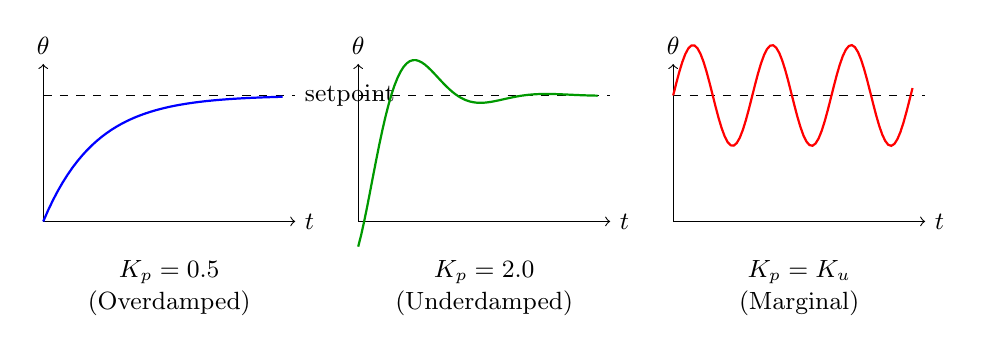
\begin{tikzpicture}[scale=0.8]
  % Low gain - stable
  \begin{scope}[shift={(-5,0)}]
    \draw[->] (0,0) -- (4,0) node[right] {\small $t$};
    \draw[->] (0,0) -- (0,2.5) node[above] {\small $\theta$};
    \draw[dashed] (0,2) -- (4,2) node[right] {\small setpoint};
    \draw[blue,thick,domain=0:3.8,samples=50] plot (\x,{2*(1-exp(-1.2*\x))});
    \node at (2,-0.8) {\small $K_p = 0.5$};
    \node at (2,-1.3) {\small (Overdamped)};
  \end{scope}

  % Medium gain - slight overshoot
  \begin{scope}[shift={(0,0)}]
    \draw[->] (0,0) -- (4,0) node[right] {\small $t$};
    \draw[->] (0,0) -- (0,2.5) node[above] {\small $\theta$};
    \draw[dashed] (0,2) -- (4,2);
    \draw[green!60!black,thick,domain=0:3.8,samples=80] plot (\x,{2*(1-1.2*exp(-1.5*\x)*cos(3*\x r))});
    \node at (2,-0.8) {\small $K_p = 2.0$};
    \node at (2,-1.3) {\small (Underdamped)};
  \end{scope}

  % High gain - oscillation
  \begin{scope}[shift={(5,0)}]
    \draw[->] (0,0) -- (4,0) node[right] {\small $t$};
    \draw[->] (0,0) -- (0,2.5) node[above] {\small $\theta$};
    \draw[dashed] (0,2) -- (4,2);
    \draw[red,thick,domain=0:3.8,samples=80] plot (\x,{2+0.8*sin(5*\x r)});
    \node at (2,-0.8) {\small $K_p = K_u$};
    \node at (2,-1.3) {\small (Marginal)};
  \end{scope}
\end{tikzpicture}
\caption{Expected motor responses at different gain settings. Left: overdamped (slow but stable). Center: underdamped (fast with overshoot). Right: marginally stable (sustained oscillation at critical gain).}
\label{fig:motor_responses}
\end{figure}

%=============================================================================
\section{Worked Examples}
\label{sec:examples}
%=============================================================================

\begin{examplebox}[Third-Order System Stability Analysis]
Determine the stability of a system with characteristic polynomial:
\begin{equation*}
P(s) = s^3 + 4s^2 + 5s + 2
\end{equation*}

\textbf{Solution:}

\textbf{Step 1:} Check necessary conditions. All coefficients are positive: $\checkmark$

\textbf{Step 2:} Construct the Routh array.

\begin{center}
\begin{tabular}{c|cc}
\toprule
$s^3$ & 1 & 5 \\
$s^2$ & 4 & 2 \\
$s^1$ & $b_1$ & 0 \\
$s^0$ & $c_1$ & \\
\bottomrule
\end{tabular}
\end{center}

Compute $b_1$:
\begin{equation*}
b_1 = \frac{4 \cdot 5 - 1 \cdot 2}{4} = \frac{20 - 2}{4} = \frac{18}{4} = 4.5
\end{equation*}

Compute $c_1$:
\begin{equation*}
c_1 = \frac{4.5 \cdot 2 - 4 \cdot 0}{4.5} = \frac{9}{4.5} = 2
\end{equation*}

The completed Routh array:
\begin{center}
\begin{tabular}{c|cc}
\toprule
$s^3$ & 1 & 5 \\
$s^2$ & 4 & 2 \\
$s^1$ & 4.5 & 0 \\
$s^0$ & 2 & \\
\bottomrule
\end{tabular}
\end{center}

\textbf{Step 3:} Count sign changes in first column: $1 \to 4 \to 4.5 \to 2$

All positive, no sign changes.

\textbf{Conclusion:} The system is \textbf{stable}. All three poles are in the LHP.
\end{examplebox}

\vspace{1em}

\begin{examplebox}[Finding the Range of Stable Gain]
For the feedback system with open-loop transfer function:
\begin{equation*}
G(s)H(s) = \frac{K}{s(s+1)(s+4)}
\end{equation*}
determine the range of $K > 0$ for which the closed-loop system is stable.

\textbf{Solution:}

The characteristic equation is $1 + G(s)H(s) = 0$:
\begin{align*}
1 + \frac{K}{s(s+1)(s+4)} &= 0 \\
s(s+1)(s+4) + K &= 0 \\
s^3 + 5s^2 + 4s + K &= 0
\end{align*}

Construct the Routh array:
\begin{center}
\begin{tabular}{c|cc}
\toprule
$s^3$ & 1 & 4 \\
$s^2$ & 5 & $K$ \\
$s^1$ & $b_1$ & 0 \\
$s^0$ & $K$ & \\
\bottomrule
\end{tabular}
\end{center}

Compute $b_1$:
\begin{equation*}
b_1 = \frac{5 \cdot 4 - 1 \cdot K}{5} = \frac{20 - K}{5}
\end{equation*}

For stability, all first-column elements must be positive. The row $s^3$ element is $1 > 0$, which is always satisfied. The row $s^2$ element is $5 > 0$, also always satisfied. The row $s^1$ element requires $\frac{20-K}{5} > 0$, giving $K < 20$. Finally, the row $s^0$ element requires $K > 0$, which is given.

\textbf{Conclusion:} The system is stable for $\boxed{0 < K < 20}$.

At $K = 20$, the system is marginally stable with poles on the imaginary axis.
\end{examplebox}

\vspace{1em}

\begin{example}[Fourth-Order System with Parameter]
\label{ex:fourth_order}
For what values of $a$ is the following polynomial stable?
\begin{equation*}
P(s) = s^4 + 2s^3 + 3s^2 + as + 5
\end{equation*}
\end{example}

\textbf{Solution:}

Construct the Routh array:
\begin{center}
\begin{tabular}{c|ccc}
\toprule
$s^4$ & 1 & 3 & 5 \\
$s^3$ & 2 & $a$ & 0 \\
$s^2$ & $b_1$ & $b_2$ & \\
$s^1$ & $c_1$ & & \\
$s^0$ & $d_1$ & & \\
\bottomrule
\end{tabular}
\end{center}

Compute elements:
\begin{align*}
b_1 &= \frac{2 \cdot 3 - 1 \cdot a}{2} = \frac{6-a}{2} \\
b_2 &= \frac{2 \cdot 5 - 1 \cdot 0}{2} = 5 \\
c_1 &= \frac{b_1 \cdot a - 2 \cdot 5}{b_1} = \frac{\frac{6-a}{2} \cdot a - 10}{\frac{6-a}{2}} = \frac{a(6-a) - 20}{6-a} = \frac{6a - a^2 - 20}{6-a} \\
d_1 &= 5 \quad \text{(from } b_2\text{)}
\end{align*}

For stability, all first-column elements must be positive. The first condition requires $b_1 = \frac{6-a}{2} > 0$, which gives $a < 6$. The second condition requires $c_1 = \frac{6a - a^2 - 20}{6-a} > 0$. Since we need $a < 6$, we have $6 - a > 0$, so the numerator must also be positive:
\begin{equation*}
6a - a^2 - 20 > 0 \Rightarrow a^2 - 6a + 20 < 0
\end{equation*}
The discriminant is $36 - 80 = -44 < 0$, and since the coefficient of $a^2$ is positive, the quadratic $a^2 - 6a + 20$ is always positive. Therefore, $c_1 < 0$ for all real $a$ when $a < 6$.

\textbf{Conclusion:} The polynomial is \textbf{unstable for all real values of $a$}.

\hfill $\blacksquare$

\vspace{1em}

\begin{example}[Row of Zeros - Auxiliary Polynomial]
\label{ex:row_zeros}
Analyze the stability of:
\begin{equation*}
P(s) = s^5 + 2s^4 + 4s^3 + 8s^2 + 3s + 6
\end{equation*}
\end{example}

\textbf{Solution:}

Begin the Routh array:
\begin{center}
\begin{tabular}{c|ccc}
\toprule
$s^5$ & 1 & 4 & 3 \\
$s^4$ & 2 & 8 & 6 \\
$s^3$ & $b_1$ & $b_2$ & \\
\bottomrule
\end{tabular}
\end{center}

Compute:
\begin{align*}
b_1 &= \frac{2 \cdot 4 - 1 \cdot 8}{2} = \frac{8-8}{2} = 0 \\
b_2 &= \frac{2 \cdot 3 - 1 \cdot 6}{2} = \frac{6-6}{2} = 0
\end{align*}

We have a row of zeros at $s^3$. This indicates symmetric root pairs.

\textbf{Form the auxiliary polynomial} from the $s^4$ row:
\begin{equation*}
A(s) = 2s^4 + 8s^2 + 6
\end{equation*}

Taking the derivative:
\begin{equation*}
\frac{dA}{ds} = 8s^3 + 16s
\end{equation*}

Replace the zero row with coefficients from $\frac{dA}{ds}$:
\begin{center}
\begin{tabular}{c|ccc}
\toprule
$s^5$ & 1 & 4 & 3 \\
$s^4$ & 2 & 8 & 6 \\
$s^3$ & 8 & 16 & 0 \\
$s^2$ & $c_1$ & $c_2$ & \\
$s^1$ & $d_1$ & & \\
$s^0$ & $e_1$ & & \\
\bottomrule
\end{tabular}
\end{center}

Continue computing:
\begin{align*}
c_1 &= \frac{8 \cdot 8 - 2 \cdot 16}{8} = \frac{64-32}{8} = 4 \\
c_2 &= \frac{8 \cdot 6 - 2 \cdot 0}{8} = 6 \\
d_1 &= \frac{4 \cdot 16 - 8 \cdot 6}{4} = \frac{64-48}{4} = 4 \\
e_1 &= 6
\end{align*}

Final Routh array:
\begin{center}
\begin{tabular}{c|ccc}
\toprule
$s^5$ & 1 & 4 & 3 \\
$s^4$ & 2 & 8 & 6 \\
$s^3$ & 8 & 16 & 0 \\
$s^2$ & 4 & 6 & \\
$s^1$ & 4 & & \\
$s^0$ & 6 & & \\
\bottomrule
\end{tabular}
\end{center}

First column: $1, 2, 8, 4, 4, 6$ --- all positive, no sign changes.

\textbf{However}, the row of zeros indicates roots on the imaginary axis. Solving $A(s) = 0$:
\begin{equation*}
2s^4 + 8s^2 + 6 = 0 \Rightarrow s^2 = \frac{-8 \pm \sqrt{64-48}}{4} = \frac{-8 \pm 4}{4}
\end{equation*}
\begin{equation*}
s^2 = -1 \text{ or } s^2 = -3 \Rightarrow s = \pm j, \pm j\sqrt{3}
\end{equation*}

\textbf{Conclusion:} The system is \textbf{marginally stable}. There are no RHP poles, but there are two pairs of poles on the imaginary axis at $s = \pm j$ and $s = \pm j\sqrt{3}$.

\hfill $\blacksquare$

\vspace{1em}

\begin{example}[Zero in First Column (Other Elements Non-Zero)]
\label{ex:zero_first_column}
Determine the number of RHP poles for:
\begin{equation*}
P(s) = s^5 + 2s^4 + 2s^3 + 4s^2 + 11s + 10
\end{equation*}
\end{example}

\textbf{Solution:}

Begin the Routh array:
\begin{center}
\begin{tabular}{c|ccc}
\toprule
$s^5$ & 1 & 2 & 11 \\
$s^4$ & 2 & 4 & 10 \\
$s^3$ & $b_1$ & $b_2$ & \\
\bottomrule
\end{tabular}
\end{center}

Compute:
\begin{align*}
b_1 &= \frac{2 \cdot 2 - 1 \cdot 4}{2} = \frac{4-4}{2} = 0 \\
b_2 &= \frac{2 \cdot 11 - 1 \cdot 10}{2} = \frac{22-10}{2} = 6
\end{align*}

Zero in first column, but $b_2 \neq 0$. Replace 0 with $\epsilon > 0$:
\begin{center}
\begin{tabular}{c|ccc}
\toprule
$s^5$ & 1 & 2 & 11 \\
$s^4$ & 2 & 4 & 10 \\
$s^3$ & $\epsilon$ & 6 & 0 \\
$s^2$ & $c_1$ & 10 & \\
$s^1$ & $d_1$ & & \\
$s^0$ & 10 & & \\
\bottomrule
\end{tabular}
\end{center}

Compute:
\begin{align*}
c_1 &= \frac{\epsilon \cdot 4 - 2 \cdot 6}{\epsilon} = \frac{4\epsilon - 12}{\epsilon} = 4 - \frac{12}{\epsilon}
\end{align*}

As $\epsilon \to 0^+$: $c_1 \to -\infty$ (large negative)

\begin{align*}
d_1 &= \frac{c_1 \cdot 6 - \epsilon \cdot 10}{c_1}
\end{align*}

As $\epsilon \to 0^+$: $d_1 \to 6$ (positive)

Examining signs as $\epsilon \to 0^+$:
\begin{center}
\begin{tabular}{c|c|c}
\toprule
Row & Element & Sign \\
\midrule
$s^5$ & 1 & + \\
$s^4$ & 2 & + \\
$s^3$ & $\epsilon$ & + \\
$s^2$ & $-\infty$ & $-$ \\
$s^1$ & 6 & + \\
$s^0$ & 10 & + \\
\bottomrule
\end{tabular}
\end{center}

Sign changes: $+ \to +$ (no), $+ \to +$ (no), $+ \to -$ (YES), $- \to +$ (YES), $+ \to +$ (no)

\textbf{Conclusion:} There are \textbf{2 sign changes}, indicating \textbf{2 poles in the RHP}. The system is unstable.

\hfill $\blacksquare$

\vspace{1em}

\begin{example}[Closed-Loop Stability from Open-Loop Transfer Function]
\label{ex:closed_loop}
A unity feedback system has open-loop transfer function:
\begin{equation*}
G(s) = \frac{K(s+2)}{(s-1)(s+3)}
\end{equation*}
Note that the open-loop system is unstable (pole at $s = +1$). For what values of $K$ is the closed-loop system stable?
\end{example}

\textbf{Solution:}

The closed-loop transfer function is:
\begin{equation*}
T(s) = \frac{G(s)}{1+G(s)} = \frac{K(s+2)}{(s-1)(s+3) + K(s+2)}
\end{equation*}

The characteristic equation is:
\begin{align*}
(s-1)(s+3) + K(s+2) &= 0 \\
s^2 + 2s - 3 + Ks + 2K &= 0 \\
s^2 + (2+K)s + (2K-3) &= 0
\end{align*}

For a second-order polynomial $s^2 + as + b$, stability requires $a > 0$ and $b > 0$:
\begin{align*}
2 + K &> 0 \Rightarrow K > -2 \\
2K - 3 &> 0 \Rightarrow K > 1.5
\end{align*}

\textbf{Conclusion:} The closed-loop system is stable for $\boxed{K > 1.5}$.

This demonstrates \textbf{feedback stabilization}: the open-loop system is unstable, but sufficiently high feedback gain stabilizes the closed-loop system.

\hfill $\blacksquare$

%=============================================================================
\section{Summary}
\label{sec:summary}
%=============================================================================

\begin{conceptbox}[Key Concepts from Chapter 6]
\begin{center}
\begin{tabular}{@{}p{3.8cm}p{9.5cm}@{}}
\toprule
\textbf{Concept} & \textbf{Description} \\
\midrule
BIBO Stability & A system is stable if every bounded input produces a bounded output. \\[0.5em]
Pole Location Criterion & An LTI system is BIBO stable if and only if all poles of its transfer function lie in the open left half-plane (Re$(s) < 0$). \\[0.5em]
Impulse Response Criterion & Stability is equivalent to $\int_0^\infty |h(t)| \, dt < \infty$. \\[0.5em]
Routh-Hurwitz Criterion & The number of RHP poles equals the number of sign changes in the first column of the Routh array. \\[0.5em]
Marginal Stability & Poles on the imaginary axis produce sustained oscillations---not BIBO stable, but bounded impulse response. \\[0.5em]
Feedback Stabilization & Properly designed feedback can stabilize an inherently unstable system (e.g., inverted pendulum, modern fighter aircraft). \\
\bottomrule
\end{tabular}
\end{center}
\end{conceptbox}

\newpage
\section{Exercises}

\begin{exercise}
For each polynomial, determine whether all roots are in the LHP:
\begin{enumerate}
\item $s^3 + 6s^2 + 11s + 6$
\item $s^3 + 2s^2 + s + 2$
\item $s^4 + 2s^3 + 3s^2 + 4s + 5$
\end{enumerate}
\end{exercise}

\begin{exercise}
A feedback system has characteristic equation $s^3 + 3s^2 + (K+2)s + 4K = 0$. Find the range of $K$ for stability.
\end{exercise}

\begin{exercise}
Apply the Routh criterion to $s^6 + 2s^5 + 8s^4 + 12s^3 + 20s^2 + 16s + 16 = 0$. If there are imaginary axis roots, find them.
\end{exercise}

\begin{exercise}
An open-loop unstable system has transfer function $G(s) = \frac{1}{s^2 - 4}$. Design a proportional controller $K$ such that the closed-loop system is stable. What is the minimum required gain?
\end{exercise}

\begin{exercise}
Consider the inverted pendulum linearized about the upward position with transfer function $G(s) = \frac{1}{s^2 - \omega_n^2}$ where $\omega_n^2 = g/\ell$. Using PD control $C(s) = K_p + K_d s$, derive conditions on $K_p$ and $K_d$ for closed-loop stability.
\end{exercise}

\begin{exercise}
\textit{(Computer Exercise)} Using MATLAB or Python, verify your Routh array calculations from Exercises 1-3 by computing the roots directly. Plot pole locations in the $s$-plane.
\end{exercise}

\begin{exercise}
A unity feedback system has open-loop transfer function $G(s) = \frac{K(s+1)}{s(s-2)(s+5)}$. The plant is open-loop unstable. Determine the range of $K$ for which the closed-loop system is stable.
\end{exercise}

\begin{exercise}
For the characteristic polynomial $s^4 + 3s^3 + 5s^2 + 4s + 2$, construct the complete Routh array. Determine whether the system is stable, marginally stable, or unstable. If unstable, state how many poles are in the RHP.
\end{exercise}

\begin{exercise}
A system has the characteristic equation $s^4 + 2s^3 + 11s^2 + 18s + 18 = 0$. Using the Routh-Hurwitz criterion, determine if any roots lie on the imaginary axis. If so, find the frequencies of oscillation.
\end{exercise}

\begin{exercise}
Explain why marginal stability is generally unacceptable in engineering practice. Provide at least three practical reasons with examples from real systems.
\end{exercise}

%=============================================================================
% References
%=============================================================================

\section*{Historical References}

\begin{enumerate}[label={[\arabic*]}]
\item J.C. Maxwell, ``On Governors,'' \textit{Proceedings of the Royal Society of London}, vol. 16, pp. 270--283, 1868.

\item E.J. Routh, \textit{A Treatise on the Stability of a Given State of Motion}. London: Macmillan, 1877.

\item A. Hurwitz, ``Ueber die Bedingungen, unter welchen eine Gleichung nur Wurzeln mit negativen reellen Theilen besitzt,'' \textit{Mathematische Annalen}, vol. 46, pp. 273--284, 1895.

\item K.Y. Billah and R.H. Scanlan, ``Resonance, Tacoma Narrows bridge failure, and undergraduate physics textbooks,'' \textit{American Journal of Physics}, vol. 59, no. 2, pp. 118--124, 1991.
\end{enumerate}

